\chapter{Introduction}
\label{chap:introduction}

\section{Motivation}

Companies such as Buy2Sell process, register, and resell industrial electronic equipment. Before an item can enter inventory, staff must enter fields such as manufacturer, product type or model, category, condition, and country of origin \cite{buy2sell-brief}. Product labels often already contain model numbers, serial numbers, manufacturing details, specifications, and barcodes, but the data must be manually transcribed. This creates a workflow bottleneck and introduces the risk of typing errors, especially when labels are photographed in workshop lighting or printed in small technical fonts.

The application is designed around the observation that the phone camera is already a strong capture device for this environment. A mobile application can support staff at the point where the item is physically handled, reduce repeated desktop entry, and preserve a human confirmation step for fields that require judgement. The project therefore focuses on a practical capture-review-send loop rather than a fully autonomous backend replacement.

\section{Objective}

The objective is to deliver a mobile-first application that converts a product-label image into a reviewed structured JSON payload. The canonical loop is Capture, Extract, Confirm, Send, and return to Capture. The system must support camera capture and gallery import, local barcode detection, provider-based vision-language extraction, deterministic merge and validation, editable confirmation, recent history, settings, and offline queueing.

\section{Scope}

The project scope is a prototype and technical foundation for the registration workflow. The receiving side is simulated through a configurable ingest endpoint, because direct access to a production registration server is outside the project boundary. Label printing, eBay resale automation, stock valuation, and full enterprise user administration are also outside scope. The application is structured so these functions can be integrated later through the same reviewed JSON payload and idempotent ingest model.

\section{Thesis Structure}

Chapter~\ref{chap:background} gives the technical background. Chapter~\ref{chap:methodology} describes the methodology and engineering workflow. Chapter~\ref{chap:analysis} analyses the industrial problem and technical constraints. Chapter~\ref{chap:requirements} lists the functional and non-functional requirements. Chapter~\ref{chap:design} explains the system design. Chapter~\ref{chap:implementation} documents the implementation. Chapter~\ref{chap:validation} presents validation and testing. Chapter~\ref{chap:conclusion} concludes the thesis and outlines future work. The appendices contain project evidence artifacts, glossary terms, risk handling, payload examples, planning evidence, Lighthouse evidence, and the automated test inventory.

\begin{figure}[htbp]
  \centering
  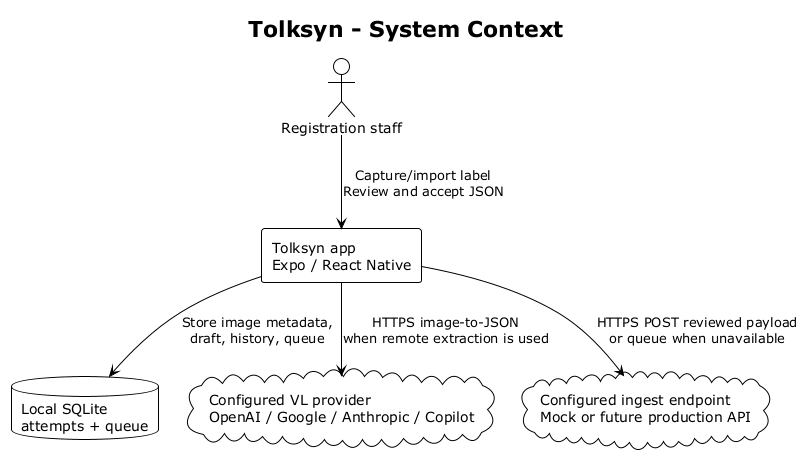
\includegraphics[width=0.92\textwidth,max height=0.58\textheight,keepaspectratio]{artifacts/system-context.png}
  \caption{System context diagram: registration staff capture a product label, review the extracted structured data, and send a JSON payload to an ingest endpoint while configured model providers handle image-to-JSON extraction.}
  \label{fig:system-context}
\end{figure}
